\documentclass[a4paper, 12pt]{article}

\usepackage[hidelinks]{hyperref}  
\usepackage{graphicx}
\usepackage{makecell}

%-----------------------

\title{\textbf{Maze Runner}}
\author{Ali-reza Iran-manesh Group 63}
\date{\today}

\begin{document}
	
\maketitle

\tableofcontents

\section{Introduction} \label{sec:introduction}
Maze Runner is a simple maze puzzle game implemented in python using terminal interface.A player suppose to find a path from entrance to the destination inside the maze structure.Once the Player reaches destination game ends.In this link you can find a game of the project uploaded on my personal Youtube account \href{https://youtu.be/eIO9C72n7Go}{(see my game preview)}.

\section{Guide} \label{sec:guide}
 The game consists of two modes;"single play" and "multi play".
 
 At the beginning, user chooses game mode.Once the mode has chosen, user should define level of difficulty of the game.This is done by choosing a number between 0-2 which represents easy,medium and hard in respective.
 \subsection{Single Play}
 The name of the user will be inserted.Now,the game has started.
 User should find his way out of the maze by starting from left bottom position where user character ,denoted by his first name letter, located at entrance.Player moves through the maze using "w" "s","a" or "d" letters to move up,down,left or right respectively and as it reaches the destination point at top right the game ends.

 \subsection{Multi Play}
 In this mode,Players input their names in order.Game starts by first player's turn.Player moves through the maze.As it reaches the end point,The time recorded and stored and other players turn initiates.
 After all players played, the results printed on terminal illustrating the winner of the game.

 At any point of game regardless of mode, user can quit the game by pressing "e" on keyboard.
  \subsection{System Requirements}
  For using this software, you need python 3.9.13 on your machine.There are no other dependencies required.
  
  Warning : It may happen that for hard level based on screen size some issues occur regarding size of the maze.
  \section{Example}
On the figure \ref{fig:figure} you can see a player inside medium sized maze trying to find his way out.
\begin{figure}
	\centering
	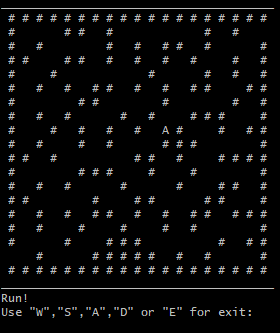
\includegraphics[width=0.8\linewidth]{maze.png}
	\caption{\label{fig:figure} Screenshot of a scene of a game in single play mode on medium level."A" refers to the player and spaces are path and "\#" are walls.}
\end{figure}

	
\end{document}